%%%%%%%%%%%%%%%%%%%%%%%%%%%%%%%%%%%
\subsection{Cameras}
\label{sec:fdgen-slow-cryo-cameras}
% glenn, jim s, chuck
% same text in single and dual phase

Cameras provide direct visual information about the state of the
detector during critical operations and when damage or unusual
conditions are suspected.  Cameras in the WA105 \(3\times 1\times
1\SI{1}{m^3}\) dual phase cryostat allowed spray from cool-down
nozzles to be seen, and the level and state of the liquid argon to be
observed as it covered the CRP \cite{Murphy:20170516}.  A camera was
used in the Liquid Argon Purity Demonstrator
cryostat\cite{Adamowski:2014daa} to study high voltage discharges in
liquid argon, and in EXO-100 during operation of a TPC
\cite{Delaquis:2013hva}.  Warm cameras viewing LAr from a distance
have been used to observe high voltage discharges in liquid argon in
fine detail \cite{Auger:2015xlo}.  Cameras are commonly used during
calibration source deployment in many experiments ({\em e.g.,} the
KamLAND ``ultra-clean'' system \cite{Banks:2014hra}).

In DUNE, cameras will be used to verify the stability, straightness,
and alignment of the hanging TPC structures during cool-down and
filling; to ensure that there is no bubbling near the ground planes
(single phase) or charge readout planes (dual phase); to inspect the
state of movable parts in the detector (calibration devices, dynamic
thermometers) as needed; and to closely inspect parts of the TPC as
necessary following any seismic activity or other unanticipated
occurrence.  These functions will be performed using set of fixed
``cold'' cameras permanently mounted at fixed points in the cryostat
for use during filling and commissioning, and a movable, replaceable
``warm'' inspection camera that can be deployed through any free
instrumentation flange at any time throughout the life of the
experiment.  Table \ref{tab:fdgen-cameras-req} summarizes the
requirements for the camera system.

\begin{dunetable}
[Camera system Requirements]
{p{0.45\linewidth}p{0.50\linewidth}}
{tab:fdgen-cameras-req}
{Camera system requirements}   
 Requirement & Physics Requirement Driver \\ \toprowrule
 {\bf General} \\ \colhline
 No component may contaminate the LAr. & High LAr purity is required for TPC operation. \\ \toprowrule
 No component may produce bubbles in the liquid argon if the HV is on. & Bubbles increase risk of HV discharge. \\ \toprowrule
 No point in the camera system shall have a field greater than \SI{15}{kV/cm} when the drift field is at nominal voltage. & Fields must be well below \SI{30}{kV/cm} to avoid risk of HV discharge.\\ \toprowrule
The camera system shall not produce measurable noise in any detector system. & Low noise is required for TPC operation. \\ \toprowrule
 Cameras will provide the viewing functionality as agreed upon with the other subsystems for viewing, as documented in the ICDs with the individual systems. \\ \toprowrule
{\bf Cold cameras} \\ \colhline
minimal heat dissipation when camera not in operation & do not generate bubbles when HV is on \\ \colhline
longevity exceeds 18 months & cameras must function throughout cryostat filling and detector commissioning \\ \colhline
Frame rate \(\geq\SI{10}{\per s}\) & observe bubbling, waves, detritus, etc. \\ \colhline
{\bf Inspection cameras} \\ \colhline
low heat transfer to LAr when in operation & do not generate bubbles, some use cases may require operation when HV is on \\ \colhline
deployable without exposing LAr to air & keep LAr free N2 and other electronegative contaminants \\ \colhline
replaceable camera enclosure & replace broken camera, or upgrade, throughout life of experiment \\ \colhline
{\bf Light emitting system} \\ \colhline
no emitted wavelength shorter than \(\SI{400}{nm}\) & avoid damaging TPB waveshifter \\ \colhline
longevity exceeds 18 months & lighting for fixed cameras must function throughout cryostat filling and detector commissioning \\ \colhline
\end{dunetable}


The following sections describe the design considerations for the cold
and warm cameras and the associated lighting system.  The same basic
design may be used for both the single and dual phase detectors.



% % % %
\subsubsection{Cryogenic Cameras (cold)}

The fixed cameras will be used to monitor the following during filling:
\begin{itemize}
\item positions of corners of APA or CRP, CPA or cathode, field cages, ground planes (~ 1 mm scale);
\item relative straightness and alignment of APA/CRP, CPA/cathode, and FC (<~ 1 mm);
\item relative position of profiles and endcaps (~ 0.5 mm)
\item state of LAr surface: is there bubbling? significant? detritus?
\end{itemize}

There are published articles and unpublished presentations describing
completely or partially successful operation of low-cost,
off-the-shelf CMOS cameras in custom enclosures immersed in cryogens.
({\em E.g.,}, EXO-100: \cite{Delaquis:2013hva}; DUNE 35-ton test
\cite{McConkey:2016spe}; WA-105: \cite{Murphy:20170516}.)  Generally
it is reported that such cameras show poor performance and ultimately
fail to function below some temperature of order \(150\sim\SI{
  200}{K}\), but some report that their cameras recover fully after
being stored (not operated) at temperatures as low as \SI{77}{K} and
then brought up to minimum operating temperature.

However, as with photon sensors, experience has also shown that it is
non-trivial to ensure reliable and reproducible mechanical and
electrical integrity of such cameras in the cryogenic environment.
({\em E.g.}, \cite{McConkey:2016spe} and
\cite{Valencia-Rodriquez:20180130}.)  Off-the-shelf cameras and camera
components are generally only specified by the vendors and original
manufactures for operation down to \SI{-40}{\celsius} or \SI{-50}{\celsius}.
In addition, many low-cost cameras use digital interfaces not intended
for long distances, such as USB (\(2\sim\SI{5}{m}\)) or CSI (circuit
board scale), leading to signal degradation and noise problems.

The design for the DUNE fixed cameras will use an enclosure based on
the successful EXO-100 design\cite{Delaquis:2013hva} which was also
used successfully in
LAPD. (Fig.\ \ref{fig:gen-fdgen-cameras-enclosure}) The enclosure will
be connected to stainless steel gas line to allow the enclosure to be
flushed with argon gas at low enough pressure to prevent
liquification, using the same design of the gas line for the beam plug
tested in the 35-ton HV test and in ProtoDUNE.  A thermocouple in the
enclosure will allow temperature monitoring, and a heating element
will provide temperature control.  The camera will transmit its video
signal using either a composite video signal over shielded coax or
ethernet over optical fiber.  Most importantly the DUNE CISC
Consortium must work with vendors to design camera circuit boards that
are robust and reliable in the cryogenic environment.

\begin{dunefigure}[A camera enclosure]{fig:gen-fdgen-cameras-enclosure}
  {CAD exploded view of vacuum-tight camera enclosure suited for cryogenic applications from \cite{Delaquis:2013hva}.
    (1) quartz window, (2 and 7) copper gasket, (3 and 6) flanges, (4) indium wires, (5) body piece, (8) signal feed-through.
  }
  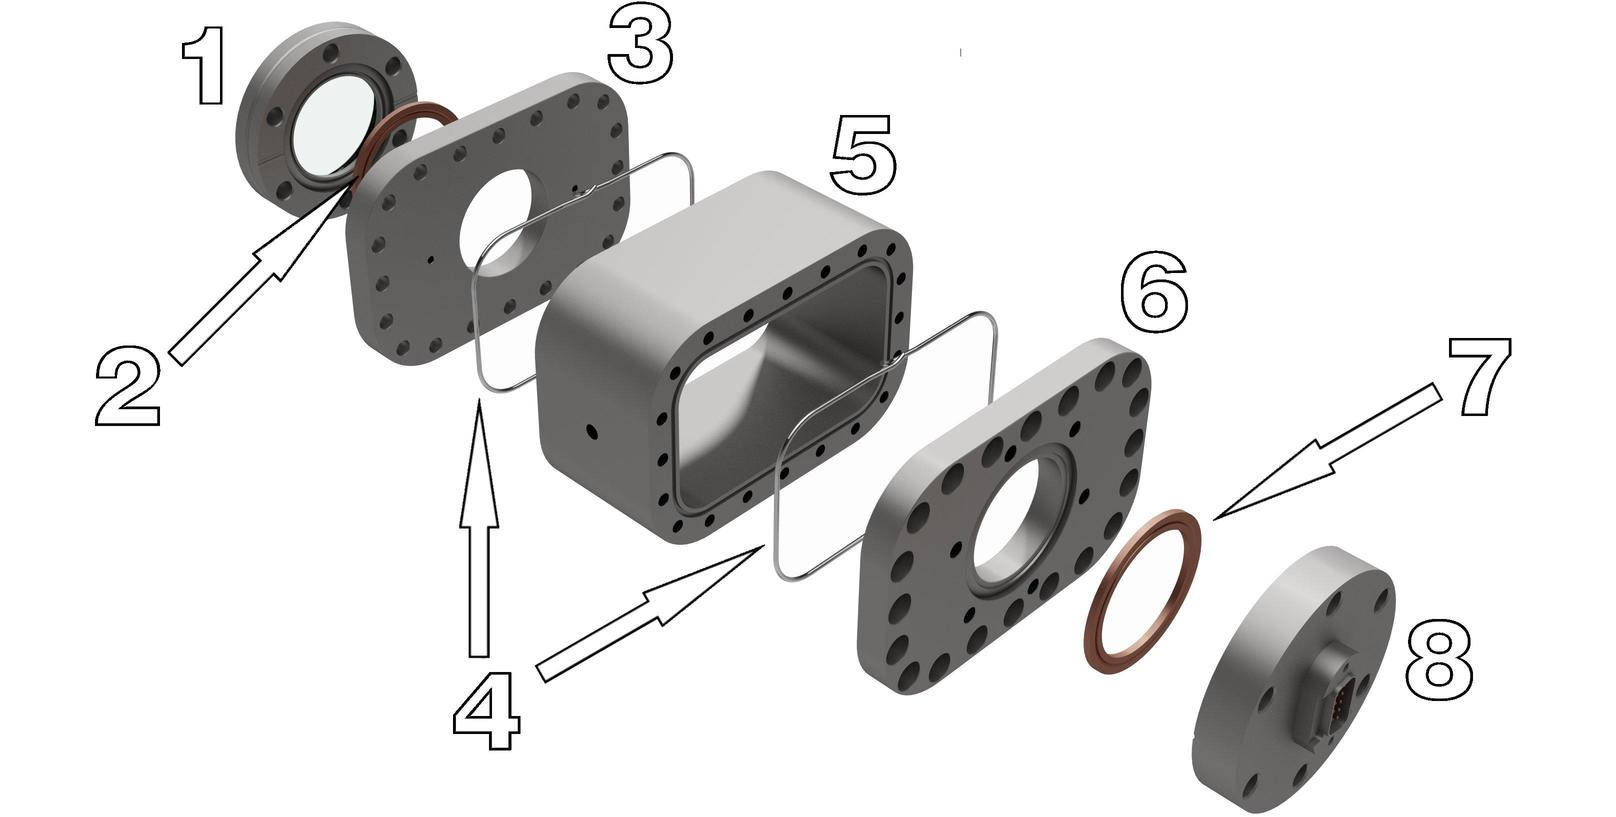
\includegraphics[width=0.6\textwidth]{exo100-camera-case}%
\end{dunefigure}



% % % %
\subsubsection{Inspection Cameras (warm)}

The inspection cameras are intended to be as versatile as possible.
However, the following locations have been identified as likely
to be of interest:
\begin{itemize}
\item Status of HV feedthrough and cup;
\item Status of profiles, endcaps (~ 0.5 mm scale);
\item Y-axis deployment of calibration sources;
\item Status of thermometers, especially dynamic thermometers;
\item HV discharge, corona, or streamers on HV feedthrough, cup, or FC;
\item relative straightness and alignment of APA/CRV, CPA/cathode, and FC (<~ 1 mm);
\item gaps between CPA frames (<~ 1 mm);
\item relative position of profiles and endcaps (~ 0.5 mm);
\item sense wires at top of outer wire planes in SP APA(~ 0.5 mm).
\end{itemize}

Unlike the fixed cameras, the inspection cameras need operate only as
long as inspection lasts, as camera replacable in case of failure.  It
is also more practical to keep the cameras continuously ``warm''
(above \SI{-150}{\celsius}) during deployment, and therefore we will
have more options for commercial cameras.  For example, we could
deploy the same model camera used successfully to observe discharges
in liquid argon from 120 cm away \cite{Auger:2015xlo}.

\begin{dunefigure}[Inspection camera design]{fig:gen-fdgen-cameras-movable}
  {An overview of the inspection camera design.}
  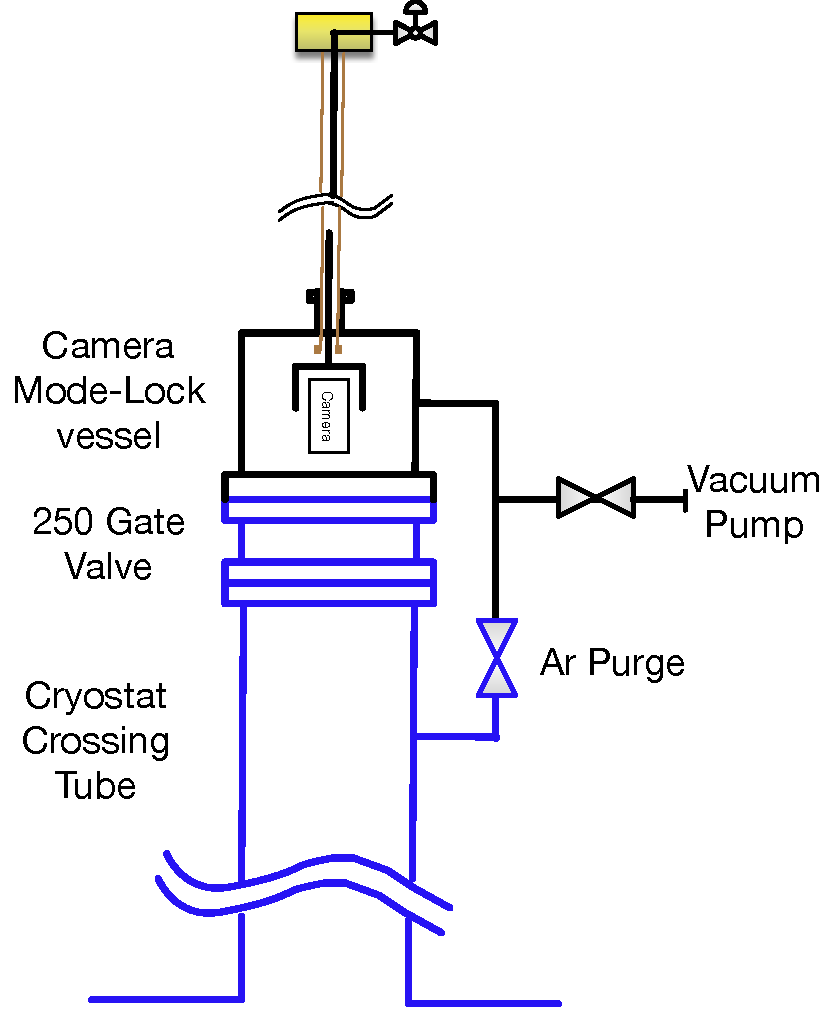
\includegraphics[width=0.3\textwidth]{Camera-Sketch}%
\end{dunefigure}

The design for the inspection camera system will use the same basic
enclosure design as for cold cameras, but mounted on an insertable
fork using a design similar to the dynamic temperature probes. (See
Fig.\ \ref{fig:gen-fdgen-cameras-movable} and
Fig.\ \ref{fig:fd-slow-cryo-sensor-mount}.)  The entire system will be sealed to
avoid contamination with air. In order to avoid contamination, the
camera can only be deployed through a feedthrough equipped with a gate
valve and a purging system, similar to that used for the vertical axis
calibration system at KamLAND\cite{Banks:2014hra}. The entire system
will be purged with pure argon gas before the gate valve is opened.

Motors above the flange will allow the fork to be
rotated and moved vertically.  A chain drive system, with motor
mounted on the end of the fork, will allow the camera assembly to be
tilted, creating a point-tilt mount with vertical motion capability.
Taking into account the room above the cryostat flanges and the
thickness of the cryostat insulation, a vertical range of motion of
\SI{1}{m} inside the cryostat is achievable.
% In the event that it
% becomes necessary to deploy a camera more deeply, we would have the
% option of building a a cable deployment system or a multi-pole
% deployment system similar to the KamLAND full-volume calibration
% system\cite{Busenitz:2009ac}, but this is not currently part of the
% baseline design.
The motors for rotation and vertical motion will be outside the sealed
volume, coupled mechanically using ferrofluidic seals, thus reducing
contamination risks and allowing for manual rotation of the vertical
drive in the event of a motor failure.  A significant protyping and
testing effort will be needed to finalize and validate this design.

% % % %
\subsubsection{Light emitting system}
%%% same text as dual-phase
The light emitting system will be based on Light-Emitting Diodes
(LEDs), with the capability of illuminating interior with selected
wavelengths (IR and visible) that are suitable for detection by the
cameras.  Performance criteria for the light emission system are based
on the efficiency of detection with the cameras, in conjunction with
adding minimal heat to the cryostat. The use of very high efficiency
LEDs will assist with the goal of reducing heat generation; as an
example, one \SI{750}{nm} LED has a specification of
32\%\ conversion of electrical input power to light.

While data on the performance of LEDs at cryogenic temperatures is sparse,
there are some studies related to NASA projects\cite{Carron:2017zzz}, which
indicate that LED efficiency increases with reduced temperature,
and that the emitted wavelengths may change, particularly for ``blue'' LEDs,
but the wavelength changes cited would have no impact on illumination, since
such short wavelength LEDs would not used, to avoid degradation of wavelength
shifting materials in the Photon Detection system.

\begin{dunefigure}[LED chain for illumination]{fig:gen-cisc-LEDs}
  {Suggested LED chain for lighting inside the cryostat, with
    dual-wavelength and failure-tolerant operation.}
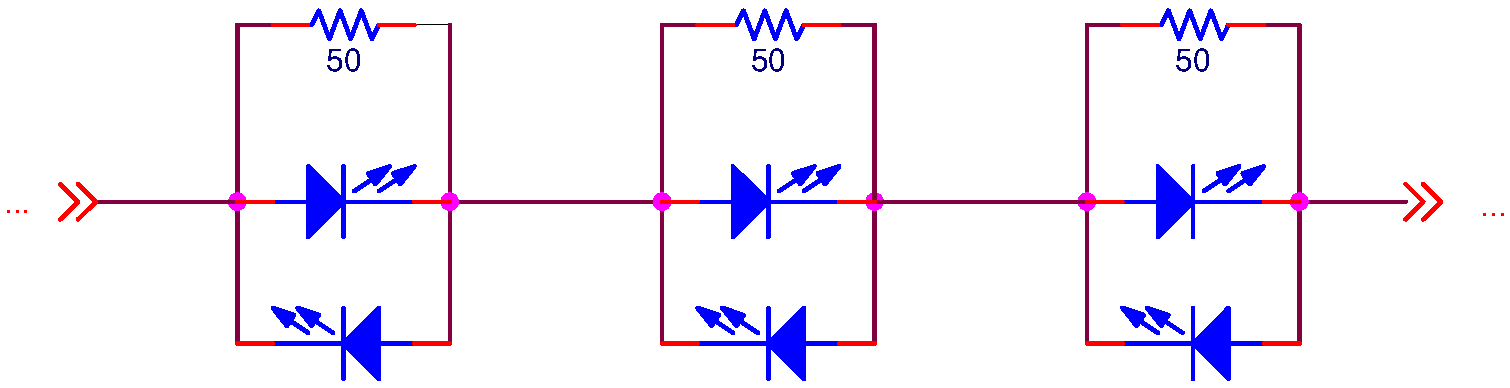
\includegraphics[width=0.7\textwidth]{CISC-Lighting}
\end{dunefigure}

A ``chain'' of LEDs should be connected in series and driven with a
constant-current circuit. It would be advantageous to pair each
LED in parallel with an opposite polarity LED and a resistor
(see Fig.~\ref{fig:gen-cisc-LEDs}).
This allows two different wavelengths of illumination with a single installed
chain (by changing the direction of the drive current) and 
continued use of an LED chain even if individual LEDs have failed.

The LEDs should be placed as a `ring light' around the outside of each
camera lens, pointing in the same direction as the lens, to 
illuminate the part of the detector within the field of
view of the camera. Commercially available LEDs can be obtained with
a range of angular spreads, so can be matched to the needs of the
cameras without additional optics. 

